\documentclass[14pt]{article}
\usepackage[utf8]{inputenc}
\usepackage[T2A]{fontenc}
\usepackage[russian]{babel} % Кириллица uchun, lekin matn lotin yozuvida
\usepackage{amsmath, amssymb}
\usepackage{geometry}
\usepackage{graphicx}
\usepackage{xcolor}
\usepackage{hyperref}
\usepackage{tasks}
\usepackage{tcolorbox}
\tcbuselibrary{skins, breakable, theorems}
\usepackage{fancyhdr}
\usepackage{lastpage}
\usepackage{enumitem}
\usepackage{paracol}
\usepackage{ifthen}
\usepackage{needspace}

% Определение команд для тангенса и котангенса (русский стиль)
\newcommand{\tg}{\operatorname{tg}}
\newcommand{\ctg}{\operatorname{ctg}}

% Настройка геометрии
\geometry{a4paper, left=10mm, right=10mm, top=20mm, bottom=20mm, headheight=15pt}

% Цветовая палитра
\definecolor{primary}{RGB}{52, 152, 219}
\definecolor{secondary}{RGB}{46, 204, 113}
\definecolor{accent}{RGB}{155, 89, 182}
\definecolor{lightbg}{RGB}{248, 249, 250}
\definecolor{taskborder}{RGB}{230, 230, 230}
\definecolor{optionbg}{RGB}{240, 242, 245}

% Основной фон страницы
\pagecolor{lightbg}

% Настройка гиперссылок
\hypersetup{
    colorlinks=true,
    linkcolor=primary,
    urlcolor=primary,
}

% Колонтитулы
\pagestyle{fancy}
\fancyhf{}
\fancyhead[L]{\textcolor{primary}{\textbf{MathCore | MOCK Test-8}}}
\fancyhead[R]{\textcolor{secondary}{Abdunazarov M.X.}}
\fancyfoot[L]{\href{https://t.me/Math_Core_Dtm_MS_Att}{\textcolor{primary}{MathCore}}}
\fancyfoot[R]{\href{https://t.me/Abd_mardon}{\textcolor{secondary}{@Abd\_mardon}}}
\fancyfoot[C]{\textcolor{gray}{\thepage/\pageref{LastPage}}}
\renewcommand{\headrulewidth}{0.5pt}
\renewcommand{\headrule}{\hbox to\headwidth{\color{primary}\leaders\hrule height \headrulewidth\hfill}}
\renewcommand{\footrulewidth}{0.5pt}
\renewcommand{\footrule}{\hbox to\headwidth{\color{secondary}\leaders\hrule height \footrulewidth\hfill}}

% Титульная страница
\title{\Huge \textbf{\textcolor{primary}{MOCK Test-8}}}
\author{\textcolor{secondary}{Abdunazarov M.X.}}
\date{}

% Стиль для карточки вопроса
\newtcolorbox{questionbox}[2][]{
    enhanced,
    breakable,
    colback=white,
    colframe=primary,
    coltitle=white,
    fonttitle=\bfseries\large,
    title={Задача \hfill \textcolor{white}{#2}},
    attach boxed title to top left={xshift=5mm, yshift=-2mm},
    boxed title style={size=small, colback=primary, sharp corners},
    sharp corners,
    boxrule=0.5pt,
    left=5mm,
    right=5mm,
    top=5mm,
    bottom=5mm,
    drop fuzzy shadow,
    #1
}

% Стиль для вариантов ответов
\newlist{options}{enumerate}{1}
\setlist[options]{
    label=\textbf{\Alph*)},
    leftmargin=*,
    itemsep=2pt,
    topsep=5pt,
    before={\vspace{2mm}\begin{tcolorbox}[
        colback=optionbg,
        colframe=white,
        sharp corners,
        boxrule=0pt,
        left=2mm,
        right=2mm,
        top=2mm,
        bottom=2mm,
    ]},
    after={\end{tcolorbox}\vspace{2mm}},
}

% Для рисунков
\newcommand{\questionimage}[2][0.5\linewidth]{%
    \begin{center}
        \includegraphics[width=#1]{#2}
    \end{center}
}

% Для удобства: команда вставки вопроса с рисунком
\newcommand{\questionitem}[4]{%
    \needspace{5cm}
    \begin{questionbox}{#1}
        #2
        \ifx&#3&%
        \else
            \questionimage{#3}
        \fi
        \begin{options}
            #4
        \end{options}
    \end{questionbox}
}

\begin{document}

% Титульная страница
\maketitle
\begin{center}
    
\includegraphics[width=0.2\textwidth]{logo.png} \\[5mm]
    \textcolor{gray}{\small Telegram: \href{https://t.me/Math_Core_Dtm_MS_Att}{@Math\_Core\_Dtm\_MS\_Att}}
\end{center}
\vspace{5mm}
% Задача 1
\begin{questionbox}{1}
    Если \(f(x) = \max\{2;\; x^2 - 1\}\), найдите значение \(f(f(0))\).
    \begin{options}
        \item 2
        \item 4
        \item 3
        \item 1
    \end{options}
\end{questionbox}


% Задача 2
\begin{questionbox}{2}
    Вычислите: \(\frac{1}{2} + 1+ \frac{3}{2} + \frac{5}{2} + 3 + ... +\frac{23}{2} +  12\).
    \begin{options}
        \item 40
        \item 56
        \item 78
        \item 150
    \end{options}
\end{questionbox}


% Задача 3
\begin{questionbox}{3}
    \(A, B, C, D, E\) — положительные целые числа, причем \(\text{НОД}(A, B, C) = 4\), \(\text{НОД}(C, D, E) = 5\). Найдите наименьшее возможное значение суммы \(A + B + C + D + E\).
    \begin{options}
        \item 22
        \item 38
        \item 36
        \item 47
    \end{options}
\end{questionbox}


% Задача 4
\begin{questionbox}{4}
    Найдите остаток от деления многочлена \(x^{1803} + 5x^{1802} + 2x^2 + 10x + 7\) на \(x + 5\).
    \begin{options}
        \item 4
        \item 5
        \item 6
        \item 7
    \end{options}
\end{questionbox}


% Задача 5
\begin{questionbox}{5}
    Если \(a < 0 < b < c\), найдите значение выражения \(\frac{|a-b| - |a| - c}{|b-a| - |a-c|}\).
    \begin{options}
        \item 1
        \item \(-1\)
        \item \(\frac{a}{c}\)
        \item \(-\frac{a}{c}\)
    \end{options}
\end{questionbox}


% Задача 6
\begin{questionbox}{6}
    Если \(a^2 + \frac{1}{a^2} = 6\), найдите значение выражения \(a^3 + \frac{1}{a^3}\).
    \begin{options}
        \item \(16\sqrt{2}\)
        \item \(10\sqrt{2}\)
        \item \(8\sqrt{2}\)
        \item \(2\sqrt{2}\)
    \end{options}
\end{questionbox}


% Задача 7
\begin{questionbox}{7}
    Сколько целых решений имеет неравенство \((2x-1)^2 (x-2)^4 (x+3)^6 (x+4)^8 \le 0\)?
    \begin{options}
        \item \(\varnothing\)
        \item 4
        \item 3
        \item бесконечно много
    \end{options}
\end{questionbox}


% Задача 8
\begin{questionbox}{8}
    Если \(2^{\log_3(x-1)} - 3^{\log_2(3-x)} = 0\), найдите \(\log_{\sqrt{2}} x\).
    \begin{options}
        \item 0
        \item \(\frac{1}{2}\)
        \item 1
        \item 2
    \end{options}
\end{questionbox}


% Задача 9
\begin{questionbox}{9}
    Сколько целых чисел удовлетворяют неравенству \(\sqrt{x^2 - 6x + 9} + \sqrt[3]{(x-2)^3} \le \sqrt[5]{(x+2)^5}\)?
    \begin{options}
        \item 9
        \item 7
        \item 8
        \item 6
    \end{options}
\end{questionbox}


% Задача 10
\begin{questionbox}{10}
    Найдите наименьший положительный период функции \(f(x) = \cos(x+5) + \operatorname{tg}^4(x+1)\).
    \begin{options}
        \item \(\frac{\pi}{4}\)
        \item \(\frac{\pi}{2}\)
        \item \(\frac{3\pi}{2}\)
        \item \(2\pi\)
    \end{options}
\end{questionbox}


% Задача 11
\begin{questionbox}{11}
    Последовательность \(8,\; 16,\; 32,\; 56,\; \dots\) обладает тем свойством, что разности соседних членов образуют арифметическую прогрессию. Найдите номер члена этой последовательности, равного 1688.
    \begin{options}
        \item 22
        \item 21
        \item 19
        \item 20
    \end{options}
\end{questionbox}


% Задача 12
\begin{questionbox}{12}
    Сколько треугольников можно образовать, принимая точки, лежащие на прямых, изображённых на рисунке, в качестве вершин?
    \begin{center}
        
\includegraphics[width=0.5\linewidth]{1.png}
    \end{center}
    \begin{options}
        \item 15
        \item 22
        \item 30
        \item 32
    \end{options}
\end{questionbox}


% Задача 13
\begin{questionbox}{13}
    В фирме работают 7 мужчин и 3 женщины. Наугад отобраны 3 человека. Какова вероятность того, что все отобранные работники — мужчины?
    \begin{options}
        \item \(\frac{3}{32}\)
        \item \(\frac{11}{28}\)
        \item \(\frac{7}{24}\)
        \item \(\frac{5}{12}\)
    \end{options}
    
\end{questionbox}


% Задача 14
\begin{questionbox}{14}
    Свободный член разложения \(\left( \sqrt{x} - \frac{2}{x} \right)^n\) равен 60. Найдите \(n\).
    \begin{options}
        \item 3
        \item 4
        \item 5
        \item 6
    \end{options}
\end{questionbox}


% Задача 15
\begin{questionbox}{15}
    Вероятность попадания в мишень для стрелка равна 0,8. Произведено 5 выстрелов. Найдите вероятность того, что первые 3 выстрела попали, а последующие 2 — нет.
    \begin{options}
        \item \(2^{10} \cdot 10^{-6}\)
        \item \(2^{11} \cdot 10^{-5}\)
        \item \(2^{11} \cdot 10^{-6}\)
        \item \(2^{10} \cdot 10^{-5}\)
    \end{options}
\end{questionbox}


% Задача 16
\begin{questionbox}{16}
    Для функции \(f(x) = \frac{g(x)+1}{3h(x)-1}\) известно, что \(g(3) = 0,\; h(3) = 2,\; h'(3) = 1,\; g'(3) = 2\). Найдите \(f'(3)\).
    \begin{options}
        \item \(\frac{5}{19}\)
        \item \(\frac{7}{19}\)
        \item \(\frac{7}{25}\)
        \item \(\frac{6}{25}\)
    \end{options}
\end{questionbox}


% Задача 17
\begin{questionbox}{17}
    На рисунке изображён график функции \(y = x^2 - 8x + m\). Известно, что \(|OB| = 3|OA|\). Найдите \(m\).
    \begin{center}
       
\includegraphics[width=0.3\linewidth]{2.png}
    \end{center}
    \begin{options}
        \item \(14\)
        \item 12
        \item 10
        \item \(6\)
    \end{options}
\end{questionbox}


% Задача 18
\begin{questionbox}{18}
    Вычислите \[\int_9^{10}(x-9)^8 xdx\]
    \begin{options}
        \item \(1\frac{1}{10}\)
        \item \(1\frac{1}{8}\)
        \item \(1\frac{1}{9}\)
        \item \(1\frac{1}{11}\)
    \end{options}
\end{questionbox}


% Задача 19
\begin{questionbox}{19}
    Если \(f(x+1)+x\cdot f(2)=x^2+3\), найдите \(f(3)\).
    \begin{options}
        \item \(3\)
        \item \(4\)
        \item \(7\)
        \item \(8\)
    \end{options}
\end{questionbox}


% Задача 20
\begin{questionbox}{20}
    Вычислите \[\int_0^{3/2}\left( \sqrt{9-x^2} - \sqrt{3}x\right)dx\]
    \begin{options}
        \item \(\frac{\pi}{2}\)
        \item \(\pi\)
        \item \(\frac{3\pi}{2}\)
        \item \(\frac{3\pi}{4}\)
    \end{options}
\end{questionbox}



% Задача 21
\begin{questionbox}{21}
    Используя приведённые данные, найдите площадь закрашенной области.
    \begin{center}
        
\includegraphics[width=0.3\linewidth]{3.png}
    \end{center}
    \begin{options}
        \item 8
        \item 10
        \item 12
        \item 14
    \end{options}
\end{questionbox}


% Задача 22
\begin{questionbox}{22}
    Какие из следующих утверждений верны?
    \begin{enumerate}
        \item Площадь круга, вписанного в треугольник, выражается формулой \(\frac{\pi}{4}\left(\frac{4S}{a+b+c}\right)^2\) (где \(a, b, c\) — стороны треугольника, \(S\) — его площадь);
        \item Отношение площадей подобных фигур равно квадрату отношения синусов соответствующих углов;
        \item Отношение объёмов конуса и цилиндра с равными высотами и радиусами оснований равно \(3\);
        \item Площадь боковой поверхности цилиндра находится по формуле \(2\pi R(R+h)\);
        \item Сумма внешних углов любого многоугольника (взятых по одному при каждой вершине) равна \(360^\circ\).
    \end{enumerate}
    \begin{options}
        \item 1,5
        \item 2,3,5
        \item 3,4
        \item 1,2,5
    \end{options}
\end{questionbox}

\vspace{1cm}

% Задача 23
\begin{questionbox}{23}
    В трапеции \(DC \parallel EF \parallel AB\), \(DC = 4\), \(AB = 2\sqrt{13}\). Найдите длину отрезка \(EF\).
    \begin{center}
        \centering
        
\includegraphics[width=0.5\linewidth]{6.png}
    \end{center}
    \begin{options}
        \item \(\sqrt{34}\)
        \item \(4\sqrt{2}\)
        \item \(\sqrt{30}\)
        \item \(2\sqrt{7}\)
    \end{options}
\end{questionbox}

\vspace{1cm}

% Задача 24
\begin{questionbox}{24}
    \(ABCD\) и \(CBFE\) — квадраты, \(AD = 6\). Найдите расстояние между точками \(O_1\) и \(O_2\) (центры квадратов).
    \begin{center}
        
\includegraphics[width=0.5\linewidth]{8.png}
    \end{center}
    \begin{options}
        \item \(2\)
        \item \(3\sqrt{3}\)
        \item \(3\)
        \item \(2\sqrt{2}\)
    \end{options}
\end{questionbox}

% Задача 25
\begin{questionbox}{25}
    На рисунке изображён правильный шестиугольник. Если \(S_{KDE} = 3\), найдите площадь закрашенной области.
    \begin{center}
      
\includegraphics[width=0.3\linewidth]{7.png}
      
    \end{center}
    \begin{options}
        \item 78
        \item 39
        \item 54
        \item 27
    \end{options}
\end{questionbox}


% Задача 26
\begin{questionbox}{26}
    Высоты треугольника равны 6, 6 и 15. Найдите площадь этого треугольника.
    \begin{options}
        \item \(90\sqrt{6}\)
        \item \(36\sqrt{15}\)
        \item \(\frac{225}{2\sqrt{6}}\)
        \item \(\frac{270\sqrt{3}}{5}\)
    \end{options}
\end{questionbox}


% Задача 27
\begin{questionbox}{27}
    Кратчайшее расстояние между окружностью \((x-a)^2 + (y-12)^2 = 25\) и прямой \(4x + 3y - 14 = 0\) равно 5. Найдите \(a\) (\(a > 0\)).
    \begin{options}
        \item 5
        \item 6
        \item 8
        \item 7
    \end{options}
\end{questionbox}


% Задача 28
\begin{questionbox}{28}
    Площадь треугольника \(ABC\) равна 12, \(BD = 3\). Найдите \(x = KC\).
    \begin{center}
       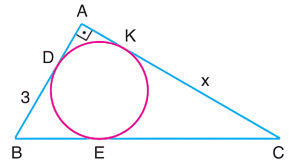
\includegraphics[width=0.5\linewidth]{21.png}
      
    \end{center}
    \begin{options}
        \item 4
        \item 5
        \item 6
        \item 7
    \end{options}
\end{questionbox}


% Задача 29
\begin{questionbox}{29}
    Боковая сторона равнобедренного треугольника равна 20, основание равно 24. Найдите расстояние от точки пересечения медиан до центра вписанной окружности.
    \begin{options}
        \item 1
        \item \(\frac{1}{3}\)
        \item \(\frac{2}{3}\)
        \item \(\frac{1}{2}\)
    \end{options}
\end{questionbox}


% Задача 30
\begin{questionbox}{30}
    В прямом цилиндре с радиусом основания 5 (рисунок) в положении I высота воды равна \(12\sqrt{3}\). Когда цилиндр наклоняют так, что его основание образует угол \(30^\circ\) с горизонтальной плоскостью (положение II), уровень воды достигает точки \(K\) на стороне \(AD\). Найдите длину \(AK\).
    \begin{center}
      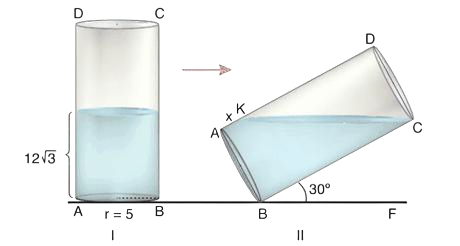
\includegraphics[width=0.5\linewidth]{22.png}
  
    \end{center}
    \begin{options}
        \item \(4\sqrt{3}\)
        \item \(5\sqrt{3}\)
        \item \(6\sqrt{3}\)
        \item \(7\sqrt{3}\)
    \end{options}
\end{questionbox}


% Задача 31
\begin{questionbox}{31}
    В прямой конический сосуд с радиусом основания 2 м и высотой 4 м (рисунок) через кран с постоянной скоростью наливают воду. Когда глубина налитой воды равна \(y\) метров, объём воды в сосуде (в \(\pi\) м\(^3\)) выражается через \(y\) как:
    \begin{center}
      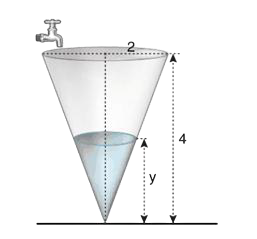
\includegraphics[width=0.5\linewidth]{32.png}
     
    \end{center}
    \begin{options}
        \item \(\frac{y^3}{3}\)
        \item \(2y^3\)
        \item \(\frac{y^3}{12}\)
        \item \(\frac{y^3}{8}\)
    \end{options}
\end{questionbox}


% Задача 32
\begin{questionbox}{32}
    Диагональ правильной четырёхугольной призмы равна \(6\sqrt{3}\). При какой высоте призмы её объём будет наибольшим?
    \begin{options}
        \item \(6\sqrt{2}\)
        \item 6
        \item \(2\sqrt{3}\)
        \item \(2\sqrt{6}\)
    \end{options}
\end{questionbox}


% Задача 33
\begin{questionbox}{33}
    Основание пирамиды — правильный шестиугольник. Высота пирамиды равна 8, сторона основания равна \(4\sqrt{3}\). Найдите апофему пирамиды.
    \begin{options}
        \item \(8\sqrt{3}\)
        \item 10
        \item \(16\sqrt{3}\)
        \item 12
    \end{options}
\end{questionbox}


% Задача 34
\begin{questionbox}{34}
    Цилиндр радиуса 6 пересечён плоскостью на расстоянии 3 от его оси. Во сколько раз площадь полученного сечения меньше площади осевого сечения?
    \begin{options}
        \item \(\sqrt{3}\)
        \item \(\frac{2\sqrt{3}}{3}\)
        \item \(\sqrt{2}\)
        \item \(\frac{3\sqrt{3}}{2}\)
    \end{options}
\end{questionbox}


% Задача 35
\begin{questionbox}{35}
    В основание конуса вписан правильный треугольник со стороной \(6\sqrt{3}\). Образующая конуса равна 10. Найдите его объём.
    \begin{options}
        \item \(48\pi\)
        \item \(72\pi\)
        \item \(96\pi\)
        \item \(36\pi\)
    \end{options}
\end{questionbox}

\end{document}